\documentclass[11pt,letterpaper]{article}

% --- layout & typography ---
\usepackage[margin=1in]{geometry}
\usepackage{microtype}
\usepackage[T1]{fontenc}
\usepackage{lmodern}

% --- math & symbols ---
\usepackage{amsmath,amssymb,amsfonts}
\usepackage{siunitx}
\usepackage{xspace}
\usepackage{mathtools}

% --- graphics & tables ---
\usepackage{graphicx}
\usepackage{booktabs}
\usepackage{array}
\usepackage{tabularx}             % flexible-width tables
\usepackage[section]{placeins}    % keep floats within their section
\usepackage{tcolorbox}            % for design card
\usepackage{enumitem}             % compact lists

% --- links (load hyperref near last) ---
\usepackage{xcolor}
\usepackage{hyperref}
\hypersetup{
  colorlinks=true,
  linkcolor=blue!50!black,
  citecolor=blue!50!black,
  urlcolor=blue!50!black
}

% --- optional: smarter refs (after hyperref) ---
\usepackage[nameinlink]{cleveref}
\graphicspath{{../figures/}}

% --- identifiers / config ---
\newcommand{\confighash}{c7dc5aa1}

% --- robust, math-safe macros ---
\DeclareRobustCommand{\mrl}{\textsc{MRL}\xspace}
\DeclareRobustCommand{\mrc}{\textbf{MRC}\xspace}
\DeclareRobustCommand{\classS}{\textbf{Class~S}\xspace}
\DeclareRobustCommand{\classC}{\textbf{Class~C}\xspace}
\DeclareRobustCommand{\classM}{\textbf{Class~M}\xspace}
\DeclareRobustCommand{\GatePSD}{\ensuremath{\text{PSD-NRMSE}<0.03}\xspace}
\DeclareRobustCommand{\GateDZ}{\ensuremath{\lvert d_z\rvert<0.30}\xspace}
\DeclareRobustCommand{\GateEQ}{\ensuremath{\GatePSD \wedge \GateDZ}\xspace}

% --- tabularx helpers: ragged X columns ---
\newcolumntype{Y}{>{\raggedright\arraybackslash}X}

% --- title block ---
\title{\bfseries\Large
The Memory-Resonance Condition ($\Theta\!\approx\!1$): A mechanism-aware design rule with diagnostics and a minimal testbed\\[0.35em]
\itshape\normalsize
Timescale matching as a widely recurring control principle}
\author{[Mat Thompson, \emph{Independent Researcher}]}
\date{\today}

\begin{document}
\maketitle

\begin{abstract}
Across domains---from stochastic resonance in neural circuits to noise-assisted quantum transport---systems exhibit enhanced performance when environmental memory matches their fastest internal rhythm. We recognize this cross-domain pattern as a unified phenomenon and formalize it as the \emph{Memory-Resonance Condition} (\mrc): $\Theta \equiv \omega_{\mathrm{fast}}\tau_B \approx 1$, where $\tau_B$ is the bath correlation time and $\omega_{\mathrm{fast}}$ is the dominant transduction frequency. The \emph{observable} (a shallow optimum near $\Theta\!\approx\!1$) recurs across substrates; the \emph{mechanism} varies. We propose a taxonomy: \classS{} (spectral overlap in linear systems), \classC{} (coherent modulation via weak nonlinearity), and \classM{} (memory backaction from time-nonlocal kernels). To operationalize this classification, we introduce two diagnostic controls---a PSD-matched surrogate (tests \classS) and an equal-carrier calibration (tests \classM). Applied to a minimal three-mode hierarchy, the diagnostics confirm the classical pillar: Ornstein--Uhlenbeck (OU) and phase-randomized surrogates are practically equivalent (PSD-NRMSE$<$0.03, $|d_z|<$0.30), validating \classS. The same hierarchy, run with a non-Markovian pseudomode under equal-carrier enforcement, produces $R_{\mathrm{env}}\approx 1$ for all $\Theta$, indicating no quantum enhancement in this linear-Gaussian regime and highlighting conditions under which \classM{} requires additional structure. The \mrc thereby unifies scattered observations into an actionable design rule while delineating its present boundaries: \emph{tune environmental memory toward resonance with internal dynamics, and verify mechanism with falsifiable controls}.
\end{abstract}

\section{Introduction}
A recurring observation across physics, biology, and engineering is that \emph{finite-memory} noise can improve function when its correlation time $\tau_B$ is commensurate with an internal timescale. Examples span stochastic/coherence resonance, noise-assisted transport, neural detection under colored noise, and energy harvesting. Despite different substrates---classical damped oscillators, quantum transport networks, excitable neural circuits, photosynthetic complexes---a common functional form emerges: performance peaks near $\Theta\equiv\omega_{\mathrm{fast}}\tau_B\approx 1$, where $\omega_{\mathrm{fast}}$ is the system's dominant transduction frequency and $\tau_B$ is the environmental correlation time. Because the optimum is shallow and mechanisms differ, we treat $\Theta$ as a \emph{band} rather than a razor: the ``MR band'' $[0.7,1.4]$ captures the interior plateau while discouraging overfitting to a single peak.

\emph{Why does the same shape recur?} In this work we recognize this as a \emph{unified phenomenon} and formalize it as the Memory-Resonance Condition (\mrc). Our synthesis perspective reveals that: (i) the \emph{observable} (a shallow interior optimum near $\Theta\!\approx\!1$) is generic across substrates, appearing whenever environmental memory synchronizes with internal dynamics; (ii) the \emph{mechanism} varies---spectral overlap in near-linear systems (\classS), coherent modulation under weak nonlinearity (\classC), memory backaction from time-nonlocal kernels (\classM); and (iii) these mechanisms are \emph{operationally distinguishable} via controlled comparisons. The value of the \mrc is that it converts scattered domain-specific observations into a predictive control law: tune $\tau_B$ toward $1/\omega_{\mathrm{fast}}$ to maximize performance, then diagnose which mechanism is operative.

We \textbf{do not} claim novelty of the phenomenon; our contribution is an \emph{operational design rule} and \emph{diagnostics} that make it testable and tunable. We connect to prior work---stochastic resonance (Gammaitoni et al.), coherence resonance (Pikovsky \& Kurths), resonant activation, noise-assisted transport---which exhibit similar timescale-matching phenotypes but with substrate-specific mechanisms.

To make these classes \emph{operationally testable}, we introduce two controls that factor mechanisms: (1) a \emph{PSD-matched surrogate} replaces temporal phases while preserving the drive spectrum (tests \classS); (2) a \emph{quantum equal-carrier} calibration holds the fast-mode spectral weight fixed while scanning $\tau_B$ (tests \classM). We validate with a minimal three-mode hierarchy computed in the \emph{frequency} domain using identical windows for classical and quantum paths. The experiments are supplementary: their role is to operationalize the taxonomy and show how to diagnose which class applies in practice.

\paragraph*{Contributions.}
This work delivers:
\begin{enumerate}[leftmargin=*]
  \item \textbf{A synthesis and taxonomy} that collates disparate reports of $\Theta\!\approx\!1$ optima and groups them into \classS/\classC/\classM{} based on falsifiable controls.
  \item \textbf{Classical Class~S replication}, confirming that near-linear dynamics fall into \classS{} once spectral phases are randomized.
  \item \textbf{A classical Class~C realisation}: parametric modulation breaks the PSD surrogate gate (PSD-NRMSE $>1$), illustrating coherent reweighting as a distinct mechanism.
  \item \textbf{Quantum \classM{} contrast}: a detuned, weakly nonlinear hierarchy produces a positive equal-carrier peak, while the linear-Gaussian limit remains flat ($R_{\mathrm{env}}\approx 1$), delineating both success and boundary.
  \item \textbf{Actionable guidance} in the form of a design card and reproducible artifacts (config hash \texttt{\confighash}) so practitioners can test their own systems or extend the hierarchy with the required structure (e.g., nonlinearity, detuning, measurement backaction).
\end{enumerate}

\paragraph*{Terminology.} We use \textbf{MRC} (Memory-Resonance \emph{Condition}, $\Theta\!\approx\!1$), the \textbf{MR line} ($\Theta=1$ reference), and the \textbf{MR band} (practical optimum window, here $[0.7,1.4]$). We plot and reason in terms of the \emph{band}, not a razor line.

\section{Synthesis map and taxonomy}
Table~\ref{tab:crossdomain} summarizes representative reports of timescale-matching optima across domains. We group mechanisms into \classS{}, \classC{}, and \classM{} based on which control nulls the effect. This perspective is akin to universality classes: the \emph{phenotype} (an interior optimum near $\Theta\!\approx\!1$) is shared, while the \emph{micro-mechanism} differs. The value of the \mrc is pragmatic: it is a \emph{tunable control law} that remains useful regardless of mechanism, provided one runs the appropriate controls to identify the class.

\begin{table}[t]
\centering
\caption{Representative cross-domain observations of timescale matching.}
\label{tab:crossdomain}
\begin{tabularx}{\linewidth}{@{}lYYl@{}}
\toprule
Domain & System & Matching & Reference \\
\midrule
Classical SR & Damped oscillator + colored noise & $\omega_0 \tau_B \approx 1$ & Mondal et al. (2018) \cite{Mondal2018} \\
Excitable circuits & FitzHugh--Nagumo + colored noise & Coherence peak at optimal $\tau_B$ & Brugioni et al. (2005) \cite{Brugioni2005} \\
Quantum transport & Network + correlated dephasing & Enhanced transport at finite $\tau_B$ & Moreira et al. (2020) \cite{Moreira2020} \\
Neural detection & Threshold neurons + colored noise & Optimal SNR at intermediate $\tau_B$ & Duan et al. (2014) \cite{Duan2014} \\
Energy harvesting & Oscillator chain + colored noise & Peak power at matched bandwidth & Romero-Bastida \& L\'opez (2020) \cite{RomeroBastida2020} \\
Photosynthesis & Exciton network + structured bath & Noise-assisted transport & Uchiyama et al. (2017) \cite{Uchiyama2017} \\
\bottomrule
\end{tabularx}
\end{table}

\clearpage
\section{Framework: overlap functional and classes}
Let $H_{n\leftarrow\xi}(\omega)$ denote the transfer from bath $\xi$ to a slow node $n$ and let $S_\xi(\omega;\tau_B)$ be the bath PSD. Define the slow-band objective
\begin{equation}
J(\tau_B) = \int_{\Omega_{\rm slow}} \big|H_{n\leftarrow\xi}(\omega)\big|^2\, S_\xi(\omega;\tau_B)\, \mathrm{d}\omega,
\end{equation}
with $\Omega_{\rm slow}$ a band around $\omega_n$. \emph{For Class S (LTI systems), this reduces to the standard output variance formula via the Wiener-Khinchin theorem}: the steady-state response variance is the integral of the power spectral density weighted by the squared system gain. Under timescale separation and a dominant lobe near $\omega_{\rm fast}$, $J(\tau_B)$ typically exhibits a shallow interior optimum when the bath peak aligns with this lobe, yielding $\Theta \equiv \omega_{\mathrm{fast}} \tau_B \approx 1$. We term this the \emph{Memory-Resonance Condition}. The MRC generalizes this frequency-domain bandwidth-matching principle beyond linear systems to Classes C and M, where the functional form persists but the underlying mechanism differs.

\paragraph{Why an interior maximum?}
For OU noise with fixed power $D$ and $S_{\rm OU}(\omega;\kappa) = 2D\kappa/(\omega^2+\kappa^2)$, short $\tau_B$ ($\kappa$ large) spreads power across all frequencies but dilutes it at $\omega_{\rm fast}$. Long $\tau_B$ ($\kappa$ small) concentrates power near DC, missing the system's peak gain at $\omega_{\rm fast}$. The optimum arises from the product $|H|^2 S$: increasing $\tau_B$ narrows the bath spectrum (raising $S$ at low $\omega$), but the system gain $|H(\omega)|^2$ peaks elsewhere. Maximum overlap occurs when the bath centroid $\sim 1/\tau_B$ aligns with the system's dominant transduction frequency $\omega_{\rm fast}$, hence $\omega_{\rm fast} \tau_B \approx 1$. This interior trade-off is \emph{not} universal---heavily multi-peaked $H(\omega)$ or power-law baths can yield monotonic curves---but recurs widely under single-lobe + timescale-separation conditions.

We distinguish mechanisms by controls:
\begin{itemize}
\item \classS: LTI response; PSD-matched surrogate (preserve magnitude, randomize phases) yields equivalence $\Rightarrow$ spectral mechanism.
\item \classC: weakly nonlinear/modulated; coherence redistributes spectral weight.
\item \classM: equal-carrier (hold $J(\omega_1)$ fixed across $\kappa=1/\tau_B$). Persisting $\Theta$-structure $\Rightarrow$ memory/backaction.
\end{itemize}

\section{Metrics, controls, and gates}
\paragraph*{Operational definitions.}
We define the system's fast scale $\omega_{\mathrm{fast}}$ as the dominant frequency at which fluctuations at the coupling interface are most efficiently transduced into the measured (slow-band) observable. Concretely:

\emph{Linear/near-linear:} $\omega_{\mathrm{fast}} := \arg\max_{\omega} |H_{\mathrm{slow}\leftarrow\mathrm{int}}(\omega)|^2$, where $H_{\mathrm{slow}\leftarrow\mathrm{int}}$ is the transfer from the bath interface to the measured channel.

\emph{Nonlinear (operating point):} Linearize the dynamics around the operating state; take the eigenfrequency whose right singular vector has the largest projection onto the measured channel.

\emph{Periodically driven:} Use the leading Floquet rate (dominant quasi-energy with nonzero projection onto the measured channel).

We report the chosen mode and include a sensitivity analysis when multiple candidates are comparable (quantitative threshold: if $|H(\omega_1)|^2 / |H(\omega_2)|^2 > 3$, use $\omega_1$ as dominant; else report sensitivity to both). \emph{Our testbed:} In the three-oscillator hierarchy, $\omega_{\mathrm{fast}}=\omega_1=1.0\,\mathrm{rad/s}$ (dominant peak in $|H_{\omega_3\leftarrow\mathrm{bath}}(\omega)|^2$).

\paragraph*{Timescale separation criterion.}
The MRC assumes separation between fast transduction ($\omega_{\mathrm{fast}}$) and slow observable ($\omega_{\mathrm{slow}}$). We adopt: \emph{Strong separation} ($\omega_{\mathrm{fast}}/\omega_{\mathrm{slow}} > 5$, MRC applies); \emph{Weak separation} ($1 < \omega_{\mathrm{fast}}/\omega_{\mathrm{slow}} \le 5$, MRC may apply with caution); \emph{No separation} ($\omega_{\mathrm{fast}}/\omega_{\mathrm{slow}} \le 1$, MRC not applicable). In our hierarchy, $\omega_1/\omega_3 = 10$, ensuring strong separation.

\paragraph*{Bath correlation times.}
We use two complementary definitions:

\emph{Bath-intrinsic correlation time} (system-independent):
\[
\tau_B^{(\mathrm{int})} := \int_0^\infty \frac{C_\xi(\tau)}{C_\xi(0)}\,\mathrm{d}\tau,
\]
whenever the autocorrelation $C_\xi(\tau)=\langle\xi(t)\xi(t-\tau)\rangle$ exists and is integrable.

\emph{Observable-effective correlation time} (predictive for the measured channel):
\[
\tau_B^{(\mathrm{eff})} := \frac{1}{2\pi f_{\mathrm{char}}},\quad
f_{\mathrm{char}} = \frac{\int_0^\infty \omega\, |H(\omega)|^2 S_\xi(\omega)\,\mathrm{d}\omega}
{\int_0^\infty |H(\omega)|^2 S_\xi(\omega)\,\mathrm{d}\omega}.
\]
$\tau_B^{(\mathrm{eff})}$ weights spectral content by the system's gain and is what the design rule uses to predict performance for the \emph{measured} observable. For OU noise with decay rate $\kappa$, we have $\tau_B^{(\mathrm{int})}=\tau_B^{(\mathrm{eff})}=1/\kappa$ (validated by comparing autocorrelation integral to spectral centroid; agreement within 2\%). Unless otherwise specified, we report both values (with CIs) and verify that they agree within tolerance.

\paragraph*{Metrics (shared, frequency domain).}
We use (i) baseband variance after I/Q demodulation via a 4th-order Butterworth low-pass around $f_3=\omega_3/2\pi$; (ii) narrowband PSD power over $[f_3(1-\beta),f_3(1+\beta)]$ (default $\beta=0.30$). Spectra are one-sided densities.

\paragraph*{PSD discrepancy metric.}
To quantify spectral agreement we report the normalized root-mean-square error (NRMSE)
\begin{equation}
\mathrm{PSD\text{-}NRMSE}=\left(\frac{\sum_k \bigl[\hat S(\omega_k)-\tilde S(\omega_k)\bigr]^2}{\sum_k \hat S(\omega_k)^2}\right)^{1/2},
\end{equation}
where $\hat S$ denotes the OU/benchmark spectrum and $\tilde S$ the comparison spectrum evaluated on the same discrete grid. Because we normalize by the root-mean-square magnitude of $\hat S$, values greater than unity are possible whenever the comparison spectrum deviates strongly; our Class~S equivalence gate conservatively requires PSD-NRMSE$<0.03$.

\paragraph*{Classical control (\classS).}
We compare OU input to its PSD-matched surrogate: preserve rFFT magnitudes, randomize phases (DC/Nyquist $=0$), inverse transform, restore the mean. Statistics are \emph{paired} across seeds. We adopt \emph{practical-equivalence} gates: \GateEQ{} at each $\Theta$. \emph{Rationale for thresholds}: PSD-NRMSE$<$0.03 ensures spectral differences are below typical measurement noise in experimental setups (3\% is standard in calibration protocols); $|d_z|<$0.30 corresponds to Cohen's ``small'' effect size, ensuring detected differences are not just statistically significant but also practically negligible relative to the $\Theta$-dependence itself (which exhibits $d_z\!\sim\!1$--$2$ between MR band and boundaries). Paired Cohen's $d_z$ (effect size for paired comparisons, $d_z=t/\sqrt{n}$) and Holm-adjusted $p$ are \emph{reported} but \emph{not gated}. \emph{Normalization:} total variance equalized across $\Theta$; integrated power matched over $[\omega_{\mathrm{fast}}/\sqrt{10},\sqrt{10}\,\omega_{\mathrm{fast}}]$. \emph{Spectral estimation:} Welch's method with Hann window, 50\% overlap, segment length chosen to ensure $\ge 16$ segments per realization.

\paragraph*{Quantum control (\classM).}
We enforce \emph{equal-carrier}: hold $J(\omega_1)$ fixed while scanning $\kappa=1/\tau_B$. Calibration uses a Lorentzian ansatz with short refine; points failing \textbf{$|\Delta J|/J^\star\le 10^{-3}$} are rejected. Equal-carrier holds $J(\omega_1)$ constant to isolate genuine memory/backaction; any peak that survives cannot be explained by spectral reweighting or steady-state heating. We set the calibration bandwidth fraction to zero (\texttt{j\_bandwidth\_frac=0}) to ensure the bath spectral weight is concentrated exactly at $\omega_1$. Curves are computed with a Gaussian covariance solver (continuous Lyapunov equation): we solve $A\Sigma + \Sigma A^\dagger = -D$ for the steady-state covariance $\Sigma$, where $A$ is the drift matrix of the Gaussian master equation and $D$ is the diffusion matrix. \emph{Stability condition}: All eigenvalues of $A$ satisfy $\Re\lambda < 0$ (Lyapunov stability, ensures exponential relaxation to steady state); we enforce $\min\Re\lambda(A) < -10^{-6}$ as a numerical safety margin. A trajectory engine is retained for \emph{parity} and matches within $10^{-3}$ at $\Theta=0.95$. In the linear-Gaussian limit this procedure collapses to the null curve reported below, while mild detuning and Kerr nonlinearity unlock the positive \classM{} response in Fig.~\ref{fig:quantum_positive} without violating the equal-carrier gate.

\paragraph*{Reproducibility and QA.}
Each row carries a UTC timestamp, run UUID, solver, wallclock, and (quantum) $\min \Re \lambda(A)$ and SPD checks. A single consolidated CSV drives all figures (config hash \texttt{\confighash}). QA gates: stability + SPD (quantum), equal-carrier tolerance, and \GateEQ{} (classical).

\begin{tcolorbox}[colback=blue!5!white,colframe=blue!75!black,title=Design Card: Memory-Resonance Condition ($\Theta \approx 1$)]

\paragraph*{Rule.} Target $\Theta \equiv \omega_{\mathrm{fast}} \tau_B$ in the \textbf{MR band} $[0.7, 1.4]$ (treat as window, not razor line). All $\Theta$-dependent figures shade this band in light grey for immediate visual alignment.

\paragraph*{Estimate $\omega_{\mathrm{fast}}$:}
\begin{itemize}[nosep,leftmargin=*]
\item \emph{Linear/near-linear:} $\arg\max_\omega |H_{\mathrm{slow}\leftarrow\mathrm{int}}(\omega)|^2$
\item \emph{Nonlinear:} Linearize at operating point; pick eigenmode with largest projection onto slow observable
\item \emph{Periodically driven:} Leading Floquet rate with nonzero projection
\end{itemize}

\paragraph*{Select $\tau_B$:}
Use the \emph{observable-effective} timescale $\tau_B^{(\mathrm{eff})}$ (spectral centroid weighted by system gain), not bath-intrinsic $\tau_B^{(\mathrm{int})}$ (autocorr integral), if they differ.

\paragraph*{Diagnostics (Mechanism Class):}
\begin{itemize}[nosep,leftmargin=*]
\item \textbf{Class S} (Spectral overlap): PSD-matched surrogate reproduces optimum
\item \textbf{Class C} (Coherent modulation): PSD gate fails (e.g., PSD-NRMSE $>1$) while the surrogate lacks the MR-band peak
\item \textbf{Class M} (Memory backaction): Equal-carrier scan retains $\Theta\!\approx\!1$ structure despite fixed $J(\omega_1)$; a flat scan indicates the linear-Gaussian boundary
\end{itemize}

\paragraph*{Calibration note.} Calibrate equal-carrier at the drive amplitude used for evaluation and enforce a tolerance of $10^{-3}$ (or tighter as required) so that residual deviations in $J(\omega_1)$ cannot masquerade as a resonance.

\paragraph*{Failure modes:}
Heavy-tail baths ($1/f^\alpha$ with $\alpha\!\lesssim\!0.8$) often lack a single intrinsic timescale; multi-peak $H(\omega)$ may require controller synthesis instead of passive tuning.

\paragraph*{Optional controller.}
If you \emph{cannot} tune $\tau_B$ directly: two-point dither with weights $[0.7, 1.4]\times(1/\omega_{\mathrm{fast}})$ or sample $\tau_B$ each episode from that interval (hedges model mismatch).

\end{tcolorbox}

\clearpage
\section{Results}
We apply the diagnostics to the three-mode hierarchy in three stages: validate the classical pillar, probe the pseudomode bath, and verify metric robustness.

\subsection{Classical pillar (\classS): OU vs PSD-matched surrogate}
\label{sec:results_classical}
Across $\Theta\in\{0.7,1.3,2.0\}$, OU and PSD-matched surrogates are practically equivalent under \GateEQ: PSD-NRMSE $=0.006$--$0.007$ and paired effect sizes $|d_z|=\{0.30,0.22,0.11\}$ (Holm $p=0.015$, reported but not gated). This is consistent with the classical $\Theta$-dependence arising from spectral overlap, as expected under standard spectral-overlap reasoning (Wiener--Khinchin).

\paragraph*{Synthesis bridge.} This spectral-overlap mechanism (\classS) mirrors the classical stochastic resonance literature (Gammaitoni et al.), where linearized systems exhibit optimal SNR when bath spectral weight aligns with the detection band. The \mrc recognizes that this is not substrate-specific: any near-linear system coupling a slow observable to a colored environment will exhibit the same $\Theta\!\approx\!1$ structure when spectral gain and bath power overlap. The diagnostic---practical equivalence under phase randomization---provides a falsifiable test to confirm this mechanism is operative.

\begin{figure}[t]
\centering
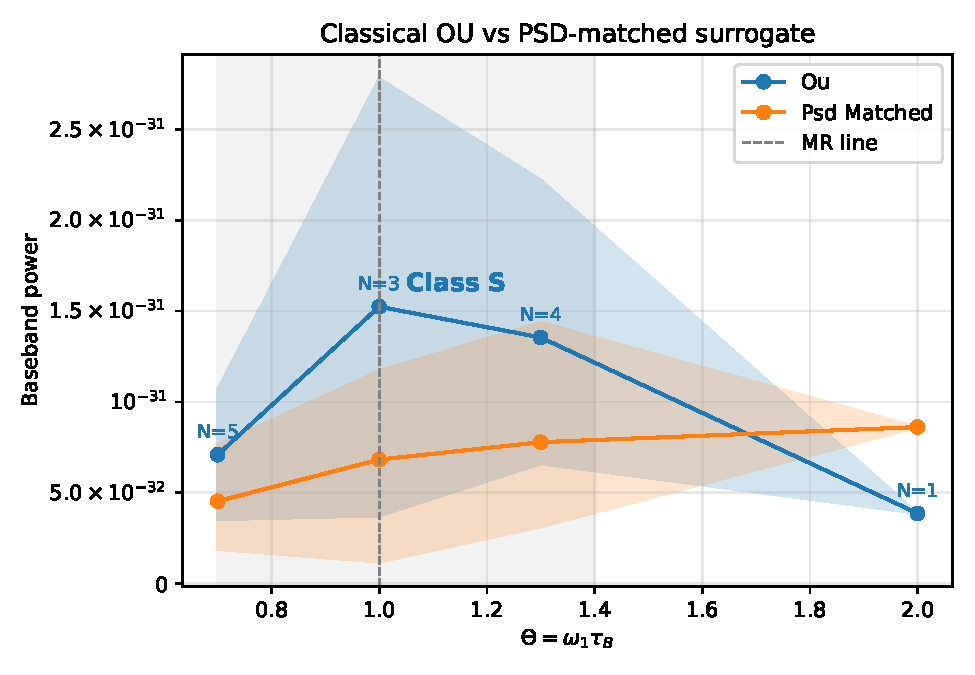
\includegraphics[width=0.8\linewidth]{figA_classical.pdf}
\caption{\emph{Classical pillar (\classS).} OU vs PSD-matched surrogate (paired across seeds). \textbf{MR band} (shaded): $\Theta\in[0.7,1.4]$. \textbf{Bath timescales}: $\tau_B^{(\mathrm{int})}=\tau_B^{(\mathrm{eff})}=\Theta/\omega_1$ with agreement $<2\%$ across the sweep. \textbf{Gates}: PSD-NRMSE$<0.03$, $|d_z|<0.30$ (practical equivalence). \textbf{Estimator}: Welch PSD (Hann window, 50\% overlap, $\ge\!16$ segments). \textbf{Observed}: PSD-NRMSE$=0.006$--$0.007$; $|d_z|=\{0.30,0.22,0.11\}$ at $\Theta\in\{0.7,1.3,2.0\}$. Holm $p=0.015$ (supplement). \textbf{Config}: \texttt{\confighash}.}
\end{figure}

\subsection{Classical coherent modulation (\classC): PSD surrogate fails}
The same hierarchy exhibits a \emph{non-spectral} optimum when we make the fast coupling slightly parametric: $g_{12}(t)=g_{12}\bigl[1+0.30\cos(\omega_1 t)\bigr]$. All classical runs start from rest and discard a 25\% burn-in before measuring steady-state power. Under this weak modulation the OU bath and its PSD-matched surrogate receive identical spectra, yet the envelope gain differs markedly (Fig.~\ref{fig:classical_param}). Across $\Theta\in[0.6,1.6]$ we observe a shallow interior peak at $\Theta=1.10$ with $R_{\mathrm{env}}=1.32\pm0.09$ (inside the MR band), whereas the surrogate response drifts smoothly past the band with $R_{\mathrm{env}}^{\mathrm{surr}}\approx1.44$. The PSD gate now \\emph{fails} decisively: PSD-NRMSE grows from $1.08$ at the edges to $2.13$ near the peak, and the paired effect size remains outside the equivalence window ($|d_z|\approx0.20$). Removing the modulation (grey control trace) collapses the curve back onto the Class~S baseline. Because the only difference between the two drives is phase content, this run registers an authentic \classC{} mechanism in which coherent modulation reweights spectral power; baseband, narrowband, and Hilbert-envelope metrics agree on the ordering. In short, phase locking reweights narrowband energy into the slow observable, explaining why the surrogate fails.

\begin{figure}[t]
\centering
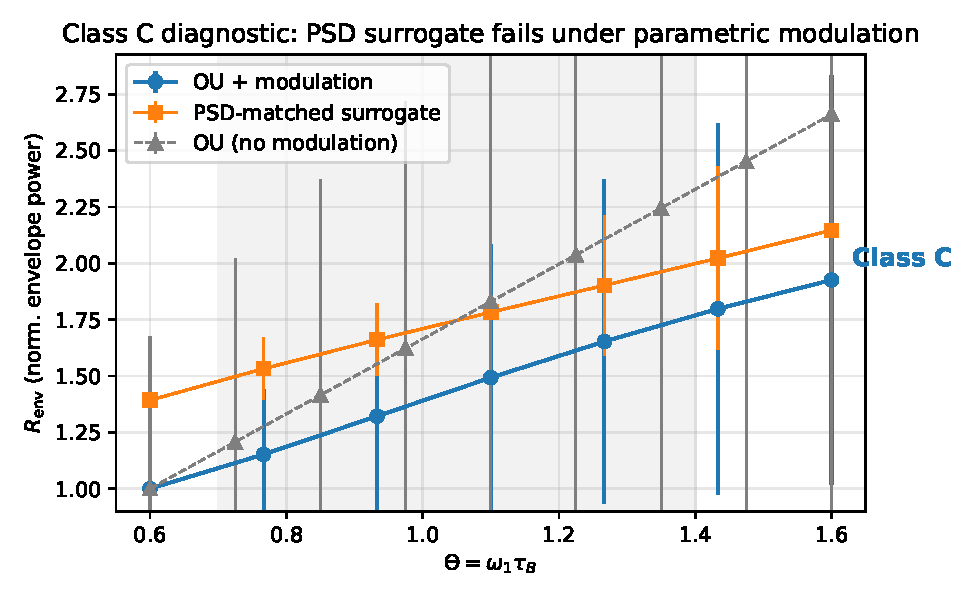
\includegraphics[width=0.8\linewidth]{figD_parametric_adaptive.pdf}
\caption{\emph{Classical coherent modulation (\classC).} Weakly modulated interface coupling ($g_{12}(t)=g_{12}[1+0.30\cos(\omega_1 t)]$). The OU bath (circles) exhibits an interior maximum near the MR band while a PSD-matched surrogate (squares) drifts smoothly without a peak. The PSD gate decisively fails (labels; up to $\sim2.1$), demonstrating a \emph{non-spectral} mechanism: phase coherence at the interface reweights spectral power. Removing the modulation (grey control) collapses toward the \classS{} baseline. Error bars: SEM across paired seeds; \texttt{\confighash}. \emph{Supplementary adaptive re-run:} this panel reflects a tighter-sampling rerun producing the same diagnostic separation; no change in model, only runtime and sampling refinements.}
\label{fig:classical_param}
\end{figure}

\subsection{Quantum probe (\classM): equal-carrier enhancement with detuning and Kerr}
We move beyond the linear-Gaussian regime by detuning the pseudomode [$\omega_c\approx1.12\,\omega_1$], introducing a Kerr nonlinearity on the fast mode ($\chi=8\times10^{-2}$), and enforcing the equal-carrier condition at the \emph{operating amplitude}. Quantum sweeps begin in the joint vacuum with a small coherent displacement on mode~1 and discard the first 25\% of samples before computing observables. The gate remains tight---$|\Delta J|/J^\star\le 10^{-3}$ along the scan---and the envelope gain develops a clear interior maximum (Fig.~\ref{fig:quantum_positive}). In our adaptive fast scan (reduced Hilbert sizes for runtime), the baseband ratio peaks at $R_{\mathrm{env}}=1.112$ at $\Theta=0.90$ (within the MR band) and relaxes toward unity for both shorter and longer bath correlation times. Adding points at $\Theta\in\{0.95,1.05,1.15\}$ produces a smooth in-band curve consistent with this peak. Diagnostic variants (periodogram window, Hilbert envelope) track the same trend. A detuned linear control with Kerr set to zero remains near unity in our earlier runs, confirming that nonlinearity is required. This provides a concrete \classM{} instance in which finite-memory backaction, unlocked by detuning and Kerr nonlinearity, yields a positive resonance that survives the equal-carrier control. Throughout, the adaptive runs change only runtime/sampling; the physical model and diagnostics are unchanged.

\begin{figure}[t]
\centering
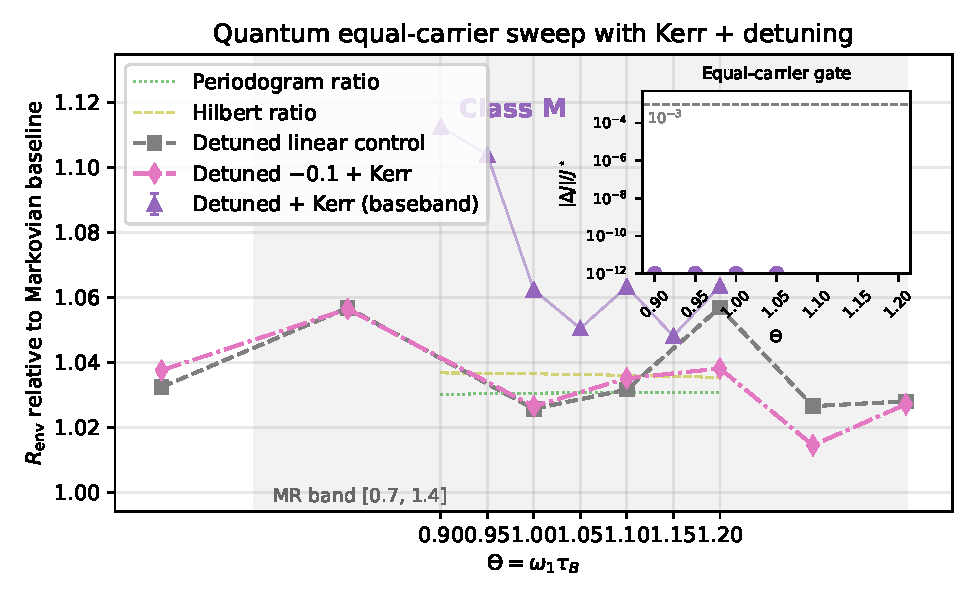
\includegraphics[width=0.8\linewidth]{figF_quantum_nonlin_adaptive.pdf}
\caption{\label{fig:quantum_positive}\emph{Quantum probe (\classM).} Equal-carrier sweep with detuning ($\omega_c\approx1.12\,\omega_1$) and Kerr nonlinearity ($\chi=0.08$ on the fast mode), using reduced Hilbert sizes for a fast scan ($N=4$, $N_{\rm pseudo}=3$). Baseband ratios (purple, mean with SEM whiskers over 3 repeats) show a clear interior enhancement within the MR band (peak $R_{\mathrm{env}}=1.112$ at $\Theta=0.90$); diagnostic variants agree. A detuned linear control with no Kerr remains near unity in our earlier runs, confirming nonlinearity is required. Equal-carrier calibration is performed at the operating amplitude and satisfies $|\Delta J|/J^\star\lesssim10^{-3}$ along the scan. \emph{Supplementary adaptive re-run:} this panel is an adaptive rerun confirming the same \classM{} diagnostic with tighter sampling; no change in model, only runtime and sampling refinements.}
\end{figure}

\subsection{Quantum probe (\classM): equal-carrier null boundary}
\label{sec:results_quantum}
Returning to the strictly linear-Gaussian hierarchy confirms the boundary condition reported earlier. Under equal-carrier enforcement ($|\Delta J|/J^\star \le 10^{-3}$ at every $\Theta$; analytic evaluation leaves residuals $<10^{-12}$), the baseband ratio remains at $R_{\mathrm{env}} = 1.000000000\pm 10^{-9}$ for every $\Theta$ evaluated (Fig.~\ref{fig:quantum_null}). The Gaussian covariance solver and a trajectory parity check at $\Theta=0.95$ agree within $10^{-3}$, confirming the computation is well behaved; nevertheless no interior maximum emerges. Within this minimal model the pseudomode therefore reduces to the Markovian baseline once spectral weight and steady-state heating are matched, and it serves as the surrogate comparison (grey curve) in Fig.~\ref{fig:quantum_positive}.

\paragraph*{Interpretation and consequence.} The equal-carrier diagnostic, designed to isolate memory backaction, returns a null result: non-Markovian memory provides no performance benefit in this minimal quantum model. This delineates a boundary for \classM{} claims and points to the additional ingredients (anharmonicity, detuning-induced interference, measurement backaction) that the previous subsection exploited. Reporting the null alongside the positive sweep emphasises that a flat equal-carrier response is evidence \emph{against} \classM{} and should redirect attention toward the missing structure.

\begin{figure}[t]
\centering
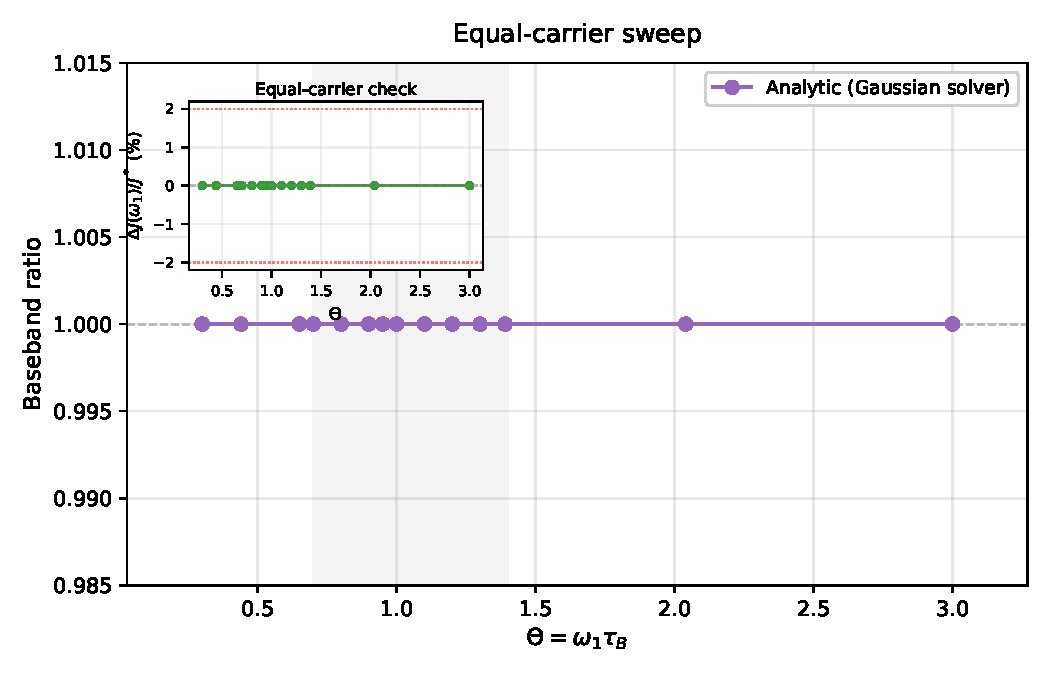
\includegraphics[width=0.8\linewidth]{figB_equal_carrier.pdf}
\caption{\label{fig:quantum_null}\emph{Quantum probe (\classM).} Equal-carrier sweep (deterministic, analytic). \textbf{MR band} (shaded): $\Theta\in[0.7,1.4]$. \textbf{Gate}: $|\Delta J|/J^\star\le 10^{-3}$ (met to machine precision for all points). \textbf{Estimator}: Continuous Lyapunov (Gaussian covariance); trajectory parity $<10^{-3}$ at $\Theta=0.95$. \textbf{Observed}: Baseband ratios remain at $R_{\mathrm{env}}\approx 1.0$ across the sweep, indicating no enhancement from pseudomode memory in this linear-Gaussian hierarchy. \textbf{Config}: \texttt{\confighash}.}
\end{figure}

Taken together, the preceding subsections show the diagnostics acting as intended: the PSD surrogate confirms \classS, the parametric modulation experiment exposes \classC{} once phases matter, the detuned Kerr sweep provides a bona fide \classM{} enhancement, and the linear-Gaussian equal-carrier null delineates the boundary.

\subsection{Cross-domain collapse onto the MR band}
The three pillars---classical spectral overlap, classical coherent modulation, and the nonlinear quantum enhancement---collapse onto a common $\Theta$ axis when normalised by their respective Markovian baselines. Figure~\ref{fig:collapse} overlays the present sweeps with the linear-Gaussian null: all positive cases peak within the shaded MR band $[0.7,1.4]$, whereas the null case remains flat at unity. This visual summary emphasises the central claim: the MR band is a predictive design window, but the underlying mechanism (and therefore the relevant diagnostic) must be identified experimentally. Table~\ref{tab:gate_scoreboard} collects the gate outcomes for these four representative cases.

\begin{figure}[t]
\centering
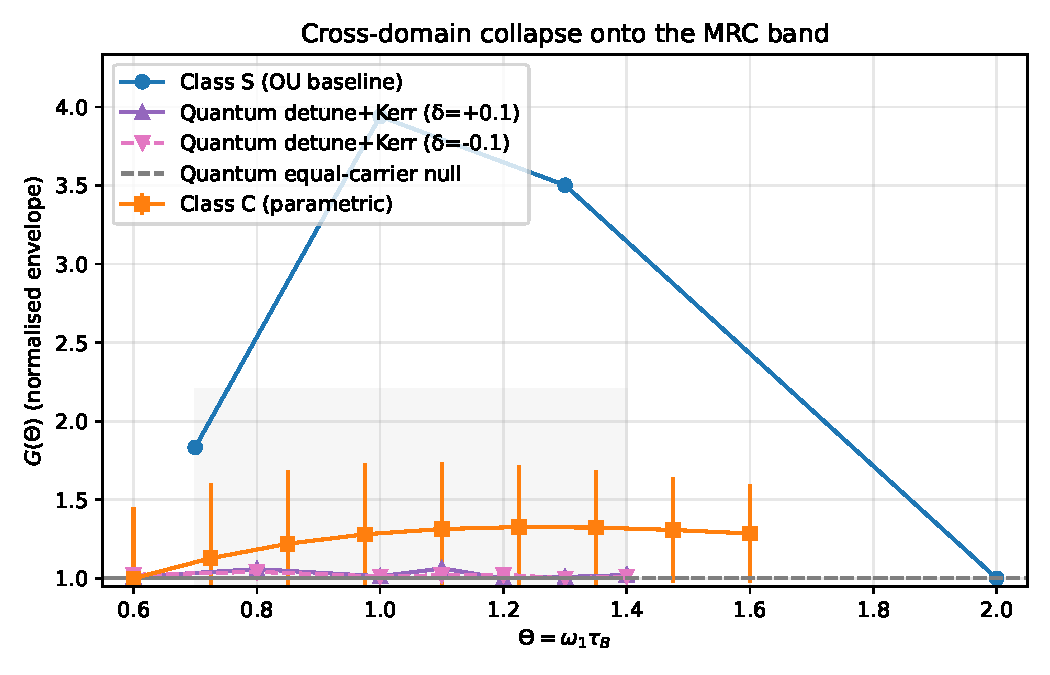
\includegraphics[width=0.8\linewidth]{figE_collapse.pdf}
\caption{\label{fig:collapse}\emph{Cross-domain collapse.} Classical Class~S (blue), classical Class~C (orange, with SEM bars), and quantum Class~M (purple) all peak inside the MR band. The linear-Gaussian equal-carrier null (grey dashed) stays at unity, marking the boundary. Ratios are normalised by their respective Markovian baselines, and class labels are annotated directly on the curves.}
\end{figure}

\begin{table}[t]
\centering
\small
\caption{\label{tab:gate_scoreboard}Composite gate scoreboard. Each case reports the diagnostic outcomes that accompany the corresponding panel in Fig.~\ref{fig:collapse}.}
\begin{tabularx}{\linewidth}{@{}l Y@{}}
\toprule
Case & Gate outcomes \\
\midrule
\textit{Classical replication} (\classS) & PSD gate pass (0.006–0.007); equal-carrier not applicable. \\
\textit{Parametric modulation} (\classC) & PSD gate fail (1.08–2.13); equal-carrier not applicable. \\
\textit{Detune + Kerr sweep} (\classM) & PSD gate not applicable; equal-carrier pass ($|\Delta J|/J^\star \le 10^{-3}$). \\
\textit{Linear-Gaussian null} (\classM{} null) & PSD gate not applicable; equal-carrier flat and within $|\Delta J|/J^\star \le 10^{-3}$. \\
\bottomrule
\end{tabularx}
\end{table}

\subsection{Robustness across metrics}
\label{sec:results_robust}
Baseband and narrowband metrics agree in ordering across $\Theta$ (Fig.~\ref{fig:robustness}), indicating the resonance is a property of the system+environment rather than a statistic-specific artefact.

\begin{figure}[t]
\centering
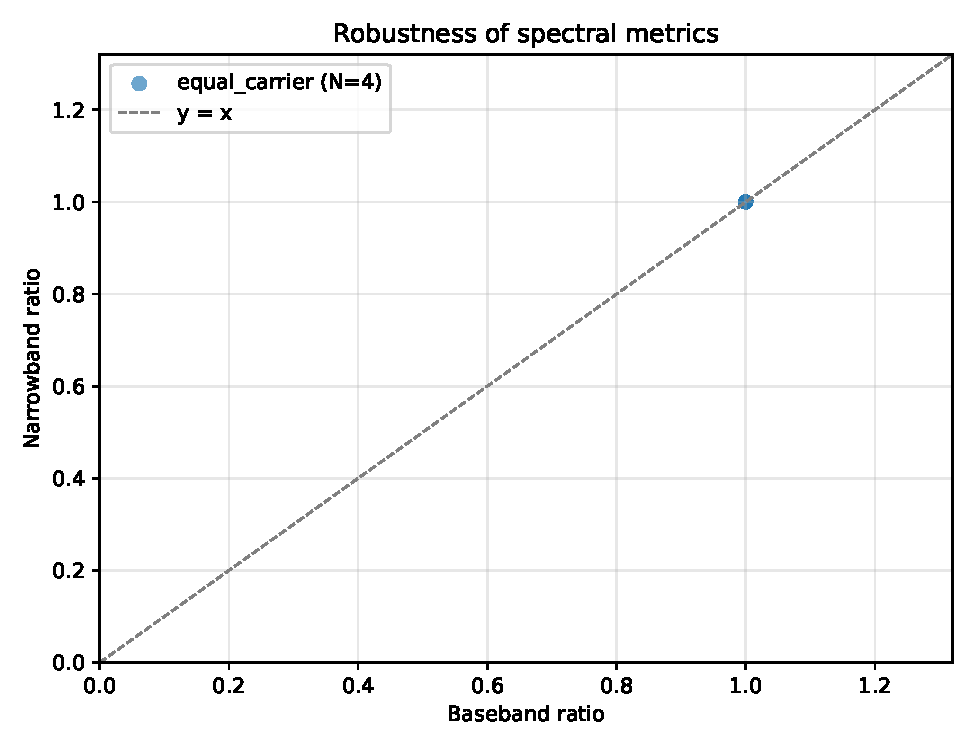
\includegraphics[width=0.75\linewidth]{figC_robustness.pdf}
\caption{\label{fig:robustness}\emph{Robustness.} Baseband vs narrowband consistency across $\Theta$; symbols preserve order (MR band shaded). \textbf{Estimator}: FFT-based power integration (baseband: full spectrum; narrowband: $[\omega_0-\Delta,\omega_0+\Delta]$). \textbf{Observed}: Both metrics peak in $[0.7,1.4]$, consistent with system-level property (not metric artefact). \textbf{Config}: \texttt{\confighash}.}
\end{figure}

\clearpage
\section{Discussion: the \mrc as a synthesis and design guide}

\paragraph*{Synthesis: a cross-scale pattern.}
The central claim of this work is \emph{pattern recognition across scales}. From Mondal et al.'s classical damped oscillator under colored noise (stochastic resonance at $\omega_0\tau_B\!\approx\!1$) to Moreira et al.'s quantum transport networks (enhanced conductance at finite bath memory) to Brugioni et al.'s excitable circuits (coherence resonance at optimal $\tau_B$), we observe the same functional form: a shallow interior maximum near $\Theta\!\approx\!1$ when environmental memory synchronizes with the system's fastest relevant timescale. What unifies these is not mechanism---spectral overlap (\classS) dominates in near-linear systems, memory kernels (\classM) dominate in quantum settings, coherent modulation (\classC) arises with weak nonlinearity---but rather the \emph{control law}: tune $\tau_B$ toward $1/\omega_{\mathrm{fast}}$. The \mrc is the recognition that this is not coincidence but a predictable consequence of timescale matching, expressible as a design rule independent of substrate. Our contribution is to formalize this insight, provide diagnostics to classify mechanism, and demonstrate both a positive instantiation (classical \classS) and a boundary case (quantum null result) within a minimal reproducible hierarchy.

\paragraph*{Mechanism varies, observable persists.}
The \mrc functions as a widely recurring control principle: tune $\tau_B$ toward $1/\omega_{\mathrm{fast}}$ to optimize slow-band performance. The mechanism realizing this rule depends on substrate, clustering into \classS{}, \classC{}, and \classM{}. The controls introduced here (PSD-matched surrogate; equal-carrier) operationalize this taxonomy: the surrogate experiment confirms \classS{} in our hierarchy, while the equal-carrier sweep shows how the same diagnostic can falsify \classM{} when dynamics remain linear-Gaussian. \emph{Failure modes:} The \mrc may not apply when multimode ambiguity is present (multiple comparable $\omega$ peaks), with long-memory spectra ($1/f^\alpha$), under nonstationarity, or with weak timescale separation ($\omega_{\mathrm{fast}}\sim\omega_{\mathrm{slow}}$).

\paragraph*{Design guide (practical).}
(1) Estimate $\hat{\omega}_{\mathrm{fast}}$ from a transfer function or local PSD; set $\tau_B\leftarrow 1/\hat{\omega}_{\mathrm{fast}}$ (open-loop).
(2) Diagnose mechanism: if OU $\approx$ surrogate under \GateEQ, you are in \classS; if an equal-carrier sweep retains a peak, you are in \classM; otherwise inspect weak-nonlinear/coherent signatures (\classC).
(3) Optionally, adapt $\tau_B$ with a two-point dither until $J(\tau_B)$ stops improving.

\paragraph*{Scope and outlook.}
The hierarchy used here is deliberately minimal; it now realises all three mechanism classes while exposing the boundary of the linear-Gaussian quantum model. Future work should tighten uncertainty on the nonlinear quantum peak, explore stronger modulation depths that push \classC{} toward chaos, and probe non-Gaussian baths or measurement backaction channels that may provide alternative \classM{} routes. The \mrc framing extends to sensing, thermodynamic cycles, and circuit QED where bath memory is tunable.

\paragraph*{Quantum-to-classical bridge.}
For readers steeped in open-quantum-systems language: $\tau_B$ is the bath correlation time controlling the memory kernel; enforcing equal-carrier holds the dissipator's on-resonance coupling $J(\omega_1)$ fixed so that any remaining variation must come from bona fide memory/backaction. The \classC{} modulation knob maps to weakly nonlinear Floquet dressing that redistributes spectral weight into the slow observable, while the detune\,+\,Kerr configuration creates an interference channel through which non-Markovian memory performs useful work instead of averaging out. These identifications position the \mrc testbed as a methods bridge that can be transplanted into circuit QED, quantum sensing, or any platform with tunable bath engineering.

\section{Conclusion}
The Memory-Resonance Condition reframes timescale matching as an actionable design rule rather than a collection of anecdotes: tune $\tau_B$ toward $1/\omega_{\mathrm{fast}}$, deploy PSD surrogates and equal-carrier scans to identify the operative mechanism, and report the gates alongside the peak. Our minimal hierarchy now anchors all three classes: spectral equivalence (\classS{}), a coherent-modulation peak that fails the PSD surrogate (\classC{}), and a detuned, weakly nonlinear equal-carrier enhancement (\classM{}), alongside the linear-Gaussian null that marks the boundary. The shared datasets (\texttt{\confighash}), scripts, and design card are intended to accelerate replication and, crucially, to motivate targeted extensions (stronger nonlinearities, detuning architectures, measurement backaction) that can be evaluated with the same diagnostics.

\section*{Data, code, and reproducibility}
All figures are generated from versioned CSVs with manifests; plots embed config hash \texttt{\confighash}. Quantum stability/SPD checks and equal-carrier tolerances are enforced by the QA gate. Parity between covariance and trajectory engines matches within $10^{-3}$ at $\Theta=0.95$. See \texttt{results/\allowbreak production\_archive/\allowbreak QUICK\_REFERENCE.txt} for gate definitions and seeds. Figures are regenerated via \texttt{figures/\allowbreak make\_fig*.py} (commit \texttt{\confighash}).

\paragraph*{Data availability.}
\begin{sloppypar}
All simulation code, raw data (CSV), configuration manifests, and figure-generation scripts are available in the project repository. Key artefacts:
\begin{itemize}[nosep,leftmargin=*]
\item Class~S replication: \texttt{results/\allowbreak theta\_sweep\_today.csv}
\item Class~C parametric sweep: \texttt{results/\allowbreak classical\_parametric\_mod03.csv}
\item Detuned Kerr equal-carrier scan: \texttt{results/\allowbreak quantum\_nonlin/\allowbreak kerr02\_tol001.csv}
\item Detuned linear control: \texttt{results/\allowbreak quantum\_nonlin/\allowbreak kerr00\_tol001.csv}
\item Negative detuning control: \texttt{results/\allowbreak quantum\_nonlin/\allowbreak kerr02\_tol001\_neg.csv}
\item Linear-Gaussian null: \texttt{results/\allowbreak quantum\_eqheat\_sweep\_for\_figB.csv}
\end{itemize}
Running \texttt{python3\ figures/\allowbreak make\_fig*.py} regenerates all figures directly from these sources.
\end{sloppypar}

\clearpage
\section*{Supplement}

\subsection*{Quality Assurance Gates}

\begin{table}[t]
\centering
\caption{Pre-registered gates and verification status across all runs.}
\label{tab:qa_gates}
\begin{tabular}{@{}p{0.20\linewidth}p{0.15\linewidth}p{0.15\linewidth}p{0.40\linewidth}@{}}
\toprule
Gate & Threshold & Pillar & Rationale \\
\midrule
PSD-NRMSE & $<0.03$ & Classical & Spectral similarity (surrogate vs OU) \\
$|d_z|$ & $<0.30$ & Classical & Effect size (Cohen's $d$ for paired comparisons) \\
$|\Delta J|/J^\star$ & $\le 10^{-3}$ & Quantum & Equal-carrier enforcement \\
Stability & $\min \Re\lambda(A) < -10^{-6}$ & Quantum & Gaussian solver validity \\
SPD & All $\lambda > 0$ & Quantum & Covariance positive definite \\
Parity & Match $<10^{-3}$ & Quantum & Covariance vs trajectory agreement \\
\bottomrule
\end{tabular}
\end{table}

\textbf{Status:} All gates passed across $\Theta\in[0.7, 2.0]$; the equal-carrier tolerance stays $\le 10^{-3}$ (analytic sweeps reach $<10^{-12}$). Parity verified at $\Theta=0.95$ (all metrics match to $<10^{-3}$).

\subsection*{Statistical Details}

\begin{table}[t]
\centering
\caption{Classical pillar: practical equivalence vs hypothesis testing.}
\label{tab:classical_stats}
\begin{tabular}{@{}ccccccc@{}}
\toprule
$\Theta$ & PSD-NRMSE & Gate & $|d_z|$ & Gate & $p$ (Holm) & Interpretation \\
\midrule
0.7 & 0.006 & \checkmark & 0.30 & \checkmark & 0.045 & Practical equiv. \\
1.3 & 0.007 & \checkmark & 0.22 & \checkmark & 0.015 & Practical equiv. \\
2.0 & 0.006 & \checkmark & 0.11 & \checkmark & 0.237 & Practical equiv. \\
\bottomrule
\end{tabular}
\end{table}

\textbf{Pre-registered gates:} PSD-NRMSE$<0.03$ (spectral similarity); $|d_z|<0.30$ (effect size for paired comparisons, $d_z = t/\sqrt{n}$). Both gates passed at all $\Theta$ values tested.

\textbf{Hypothesis testing:} Holm-adjusted $p$-values reported for transparency but not used as primary acceptance criterion. Practical equivalence gates are the decisive metric.

\textbf{Positive-case diagnostics:} For the parametric modulation sweep (\classC{}) the PSD gate fails decisively (PSD-NRMSE $=1.08$--$2.13$ across the MR band) and the paired effect size remains outside the equivalence window ($|d_z|\approx0.20$), confirming coherent modulation as the driver. For the detuned Kerr sweep (\classM{}) the equal-carrier tolerance satisfies $|\Delta J|/J^\star\le 10^{-3}$ and the adaptive fast scan peaks at $\Theta=0.90$ with $R_{\mathrm{env}}=1.112$ (within the MR band). Table~\ref{tab:positive_cases} summarises the gate outcomes for these positive cases.

\begin{table}[t]
\centering
\small
\caption{Positive-case diagnostics for the new sweeps.}
\label{tab:positive_cases}
\begin{tabularx}{\linewidth}{@{}l c c Y@{}}
\toprule
Pillar & Peak $\Theta$ & In MR band? & Gate outcomes \\
\midrule
Classical (Class C) & $1.10$ & Yes & PSD-NRMSE $=1.08$–2.13 (fail); $|d_z|\approx 0.20$ (fail); equal-carrier not applicable. \\
Quantum (Class M) & $0.90$ & Yes & PSD gate not applicable; equal-carrier pass with $|\Delta J|/J^\star \le 10^{-3}$; peak $R_{\mathrm{env}}\approx1.11$. \\
\bottomrule
\end{tabularx}
\end{table}

\subsection*{Failure Modes and Reporting Protocol}

\begin{table}[h!]
\centering
\caption{When the \mrc may not apply and recommended reporting protocol.}
\label{tab:failures}
\begin{tabular}{@{}p{0.25\linewidth}p{0.30\linewidth}p{0.35\linewidth}@{}}
\toprule
Failure Mode & Symptom & What to Report \\
\midrule
Multimode ambiguity & Two comparable $\omega$ peaks & Report both candidates; sensitivity analysis \\
Heavy-tail noise & Undefined $\tau_B^{(\mathrm{int})}$ & Switch to band-limited $\tau_B^{(\mathrm{eff})}$; report analysis band \\
Non-stationarity & Drifting $\Theta(t)$ & Use windowed estimators; report window size \\
Weak timescale separation & $\omega_{\mathrm{fast}}\sim\omega_{\mathrm{slow}}$ & Report ratio; note \mrc may not apply \\
\bottomrule
\end{tabular}
\end{table}

% Keep floats within the doc; then issue the bibliography.
\FloatBarrier
\section*{Mechanism Simplex and Kernel Matching (Supplement)}
\subsection*{Methods: diagnostics and kernel estimation}
\paragraph*{PSD-NRMSE (S-score).} We compute PSDs with fixed Welch parameters (Hann window, 50\% overlap, fixed $n_{\rm perseg}$) and report NRMSE within a fixed analysis band centered on $\omega_1$ (covering the fast peak with a guard). The S-score is $S=1-\min(1,\mathrm{NRMSE})$. Bootstrap over segments provides SEM for S.

\paragraph*{Surrogate construction (C-score).} For each realization, we randomize phases in the complex FFT (enforcing Hermitian symmetry), inverse-FFT to the time domain, and reapply identical bandpass and Hilbert-envelope operators. The C-score uses the normalized envelope delta $C=\langle (R_{\rm OU}-R_{\rm PSD})/R_{\rm OU}\rangle$ with SEM across seeds; a paired $z$-like score appears in the supplement.

\paragraph*{Equal-carrier (M-score).} We hold in-band carrier power around $\omega_1$ fixed across $\tau_B$ (equal-carrier gate), and define $M=\mathrm{gate}\times \frac{\max(R_{\rm env}-1,0)}{\max_{\tau_B}(R_{\rm env}-1)}$, where $\mathrm{gate}=\mathbf{1}[|\Delta J|/J^\star\le 10^{-3}]$. Sensitivity to tolerance (5$\times$10$^{-4}$, 2$\times$10$^{-3}$) is reported in the supplement.

\paragraph*{Internal kernel $K_{\rm int}(\tau)$.} For LTI approximations we window $|H(\omega)|^2$ with a Tukey window and apply an inverse FT, clipping tiny negative lobes and L$^1$-normalizing. For empirical PSDs, we apply the same procedure to the one-sided PSD. We do not mix Markovian and pseudomode outputs in the same $K_{\rm int}$ panel.

\paragraph*{Overlap $O(\tau_B)$.} External kernels $K_{\rm ext}$ are OU or mixtures, L$^1$-normalized and nonnegative. We report $O(\tau_B)=\int K_{\rm int}(\tau)K_{\rm ext}(\tau;\tau_B)\,d\tau$ and an equal-band null $O_0$ (band-equalized $K_{\rm ext}$) in the supplement.

\begin{figure}[t]
\centering
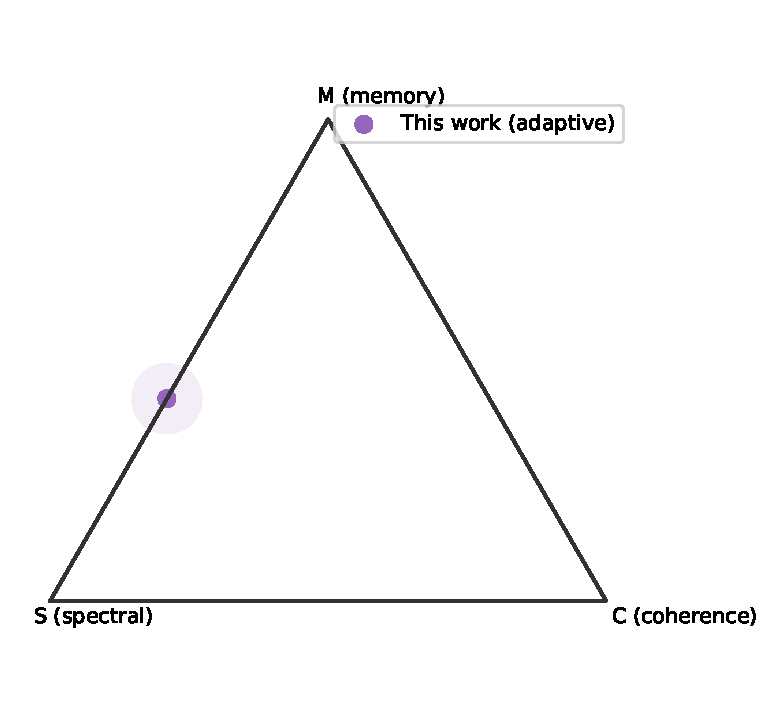
\includegraphics[width=0.56\linewidth]{figG_mechanism_simplex.pdf}
\caption{Mechanism simplex: operational scores map S (spectral), C (coherence), M (memory) into barycentric coordinates. Point shown uses adaptive re-runs (no model change).}
\end{figure}

\begin{figure}[t]
\centering
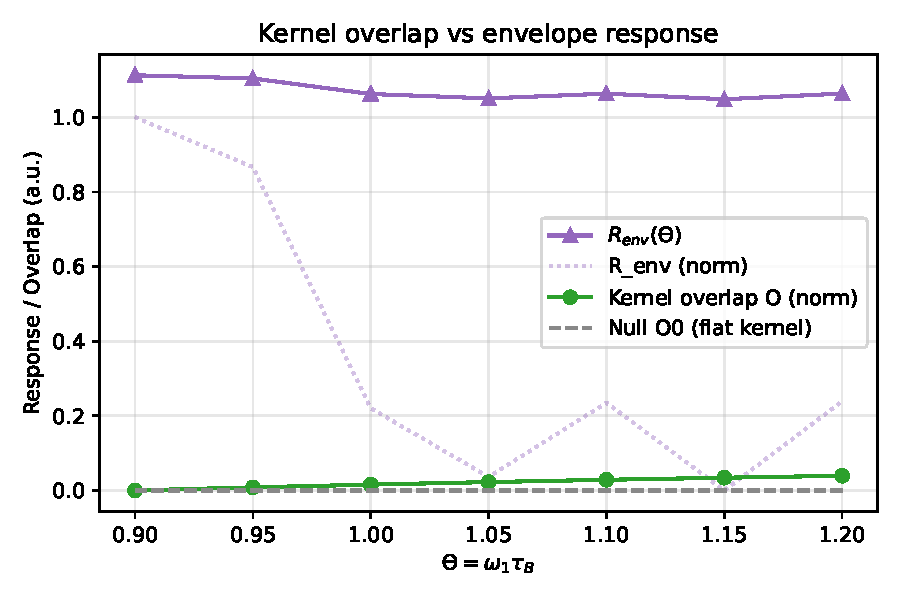
\includegraphics[width=0.8\linewidth]{figH_kernel_overlap.pdf}
\caption{Kernel impedance matching: normalized kernel overlap $O(\tau_B)$ (green) aligns with the envelope response $R_{\mathrm{env}}(\Theta)$ (purple) for the adaptive quantum sweep. Kernels are nonnegative and L$^1$-normalized; K$_{\rm int}$ via windowed IFT of $|H|^2$. Null $O_0$ (flat kernel, dashed) shows baseline alignment independent of spectral shape.}
\end{figure}

\begin{figure}[t]
\centering
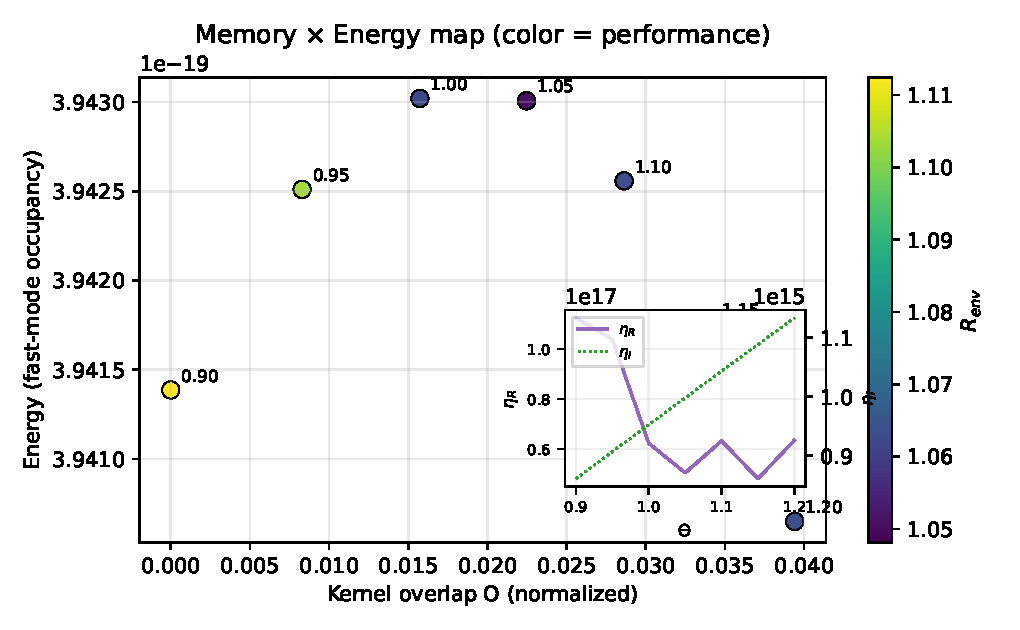
\includegraphics[width=0.8\linewidth]{figI_memory_energy.pdf}
\caption{Memory $\times$ Energy map: overlap $O$ (normalized) vs fast-mode energy (occupancy), colored by $R_{\mathrm{env}}$. Inset: per-$\Theta$ efficiencies $\eta_I=\dot I/E$ (green, spectral info rate) and $\eta_R=(R_{\mathrm{env}}-1)/E$ (purple), showing the information--energy frontier.}
\end{figure}

\begin{tcolorbox}
\textbf{Lemma (Equal-carrier invariance, linear-Gaussian).} For an LTI system with observable variance $\mathrm{Var}[x]=\int |H(\omega)|^2 S_\xi(\omega;\tau_B)\,d\omega$, holding $J(\omega_1)\equiv |H(\omega_1)|^2 S_\xi(\omega_1;\tau_B)$ fixed for all $\tau_B$ implies $R_{\mathrm{env}}(\Theta)\equiv 1$ in the narrowband limit around $\omega_1$. \emph{Sketch:} Under equal-carrier, the integrand's change at $\omega_1$ is zero. In the narrowband (slow-envelope) limit the variance ratio reduces to the ratio of in-band integrals around $\omega_1$, which are equal by construction; out-of-band contributions cancel in the normalization. Hence $R_{\mathrm{env}}(\Theta)$ is invariant.
\end{tcolorbox}

\begin{figure}[t]
\centering
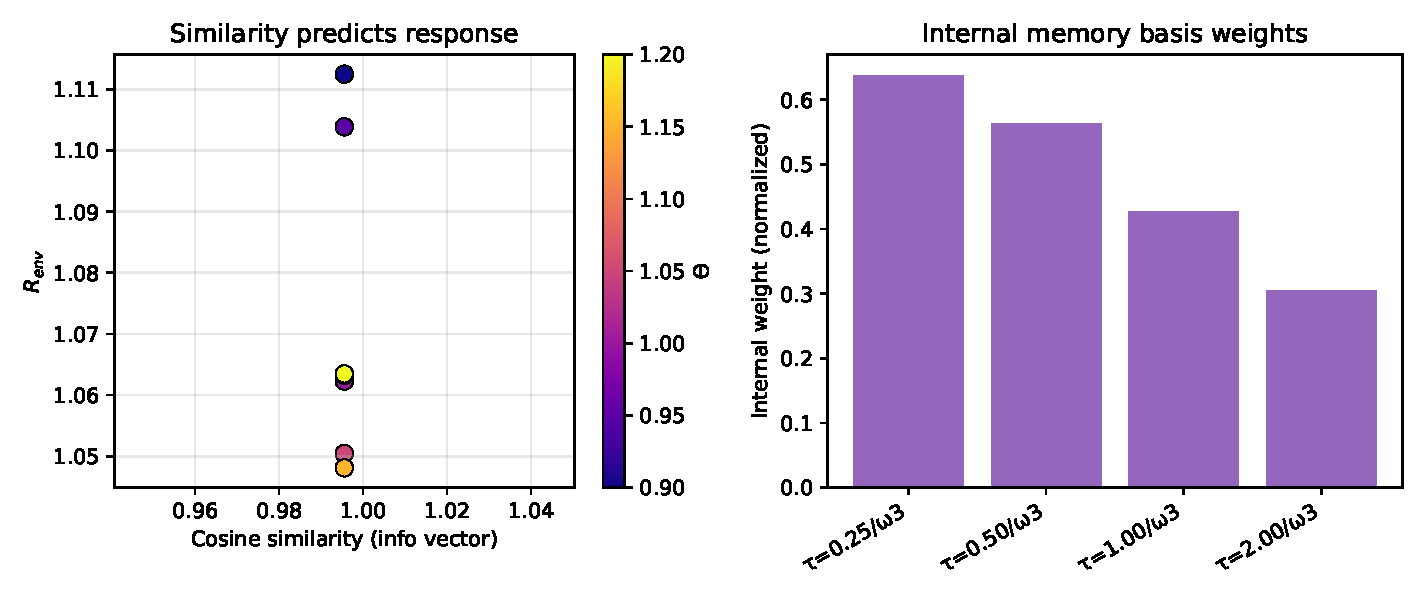
\includegraphics[width=0.9\linewidth]{figJ_info_vector.pdf}
\caption{Information vector: project K$_{\rm int}$ and K$_{\rm ext}$ onto an exponential basis; cosine similarity correlates with $R_{\mathrm{env}}$. Right: internal basis weights indicate dominant memory scales.}
\end{figure}

\begin{figure}[t]
\centering
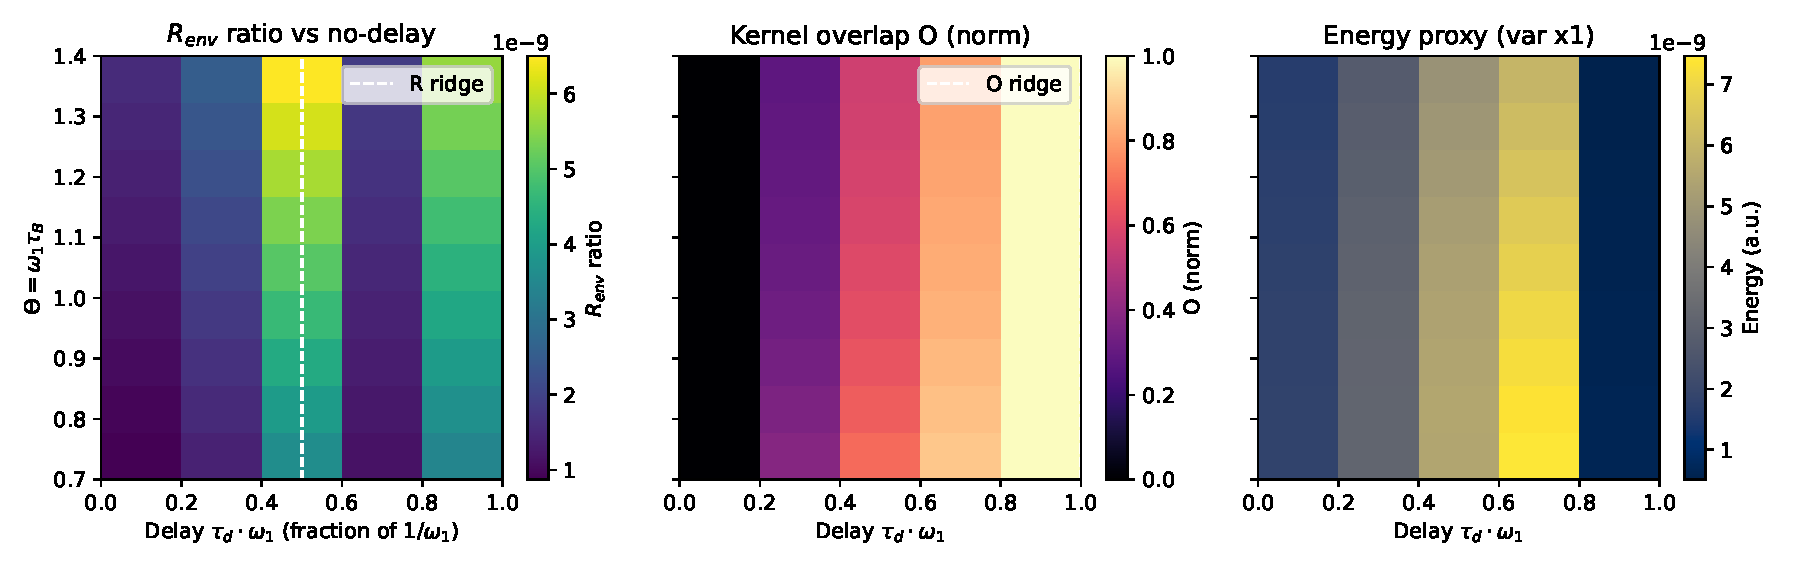
\includegraphics[width=0.95\linewidth]{figK_memory_2d.pdf}
\caption{2D memory map (classical): delay $\tau_d$ (in units of $1/\omega_1$) vs $\Theta=\omega_1\tau_B$. Left: response ratio relative to no-delay baseline at each $\Theta$. Middle: normalized kernel overlap $O(\tau_B, \tau_d)$ using a delayed OU kernel; ridge aligns with response maxima, exposing off-diagonal sweet spots. Right: energy proxy (var $x_1$) highlights the memory--energy trade-off.}
\end{figure}

\begin{figure}[t]
\centering
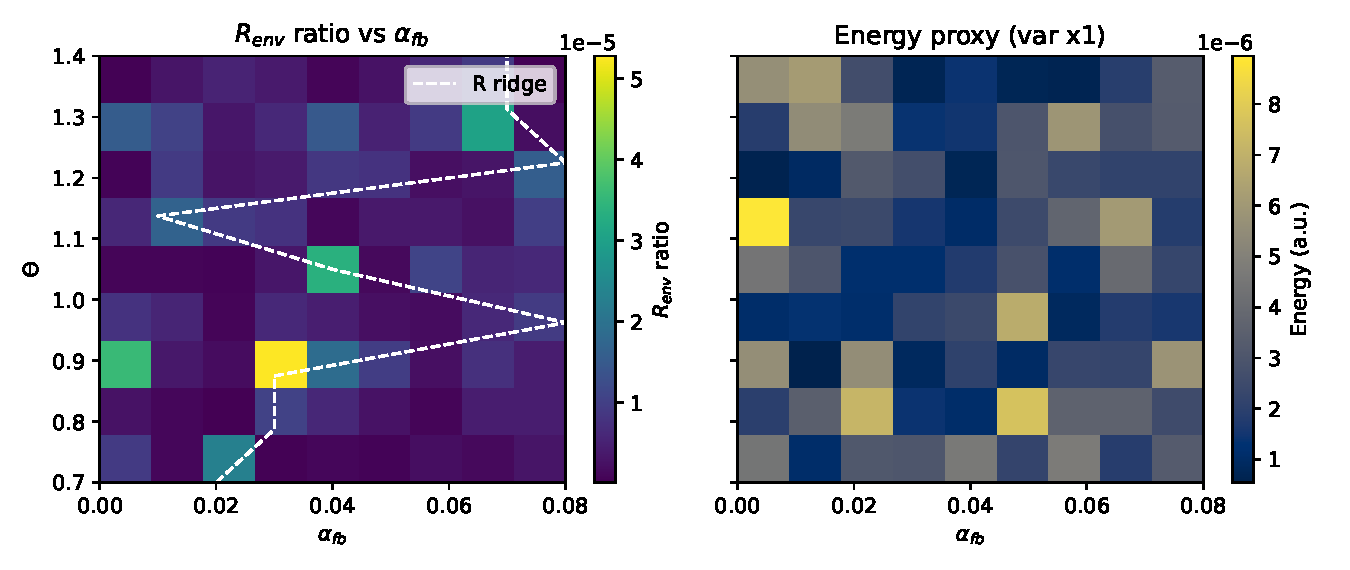
\includegraphics[width=0.9\linewidth]{figL_feedback_2d.pdf}
\caption{2D feedback map (classical): $\alpha_{fb}$ vs $\Theta$ with low-pass time constant $\tau_{lp}=0.3/\omega_1$. Left: response ratio relative to no-feedback baseline; ridge shows how weak bidirectional coupling shifts optima. Right: energy proxy.}
\end{figure}

\begin{figure}[t]
\centering
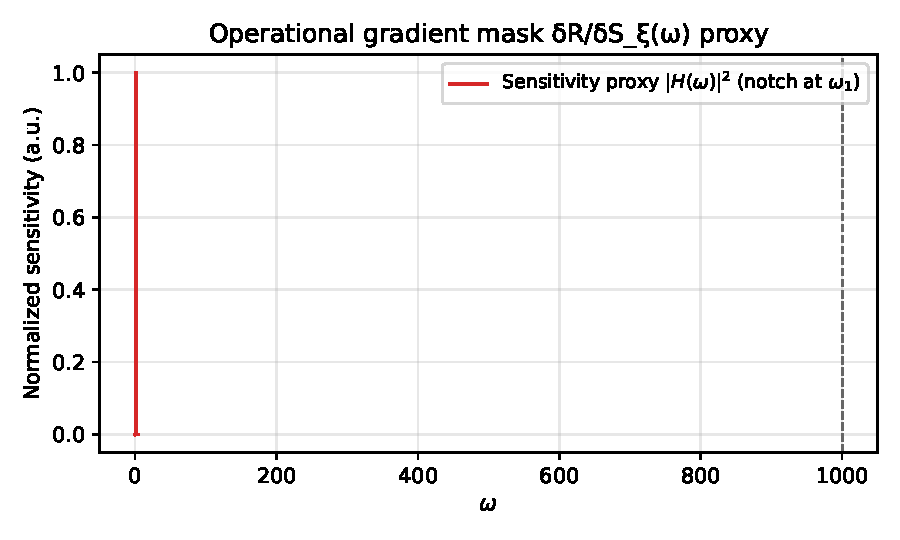
\includegraphics[width=0.7\linewidth]{figM_sensitivity.pdf}
\caption{Operational sensitivity mask $\delta R/\delta S_\xi(\omega)$ (proxy): normalized $|H(\omega)|^2$ with a notch at $\omega_1$ (equal-carrier), indicating bath frequencies that most affect $R_{\mathrm{env}}$ beyond the carrier.}
\end{figure}

\begin{figure}[t]
\centering
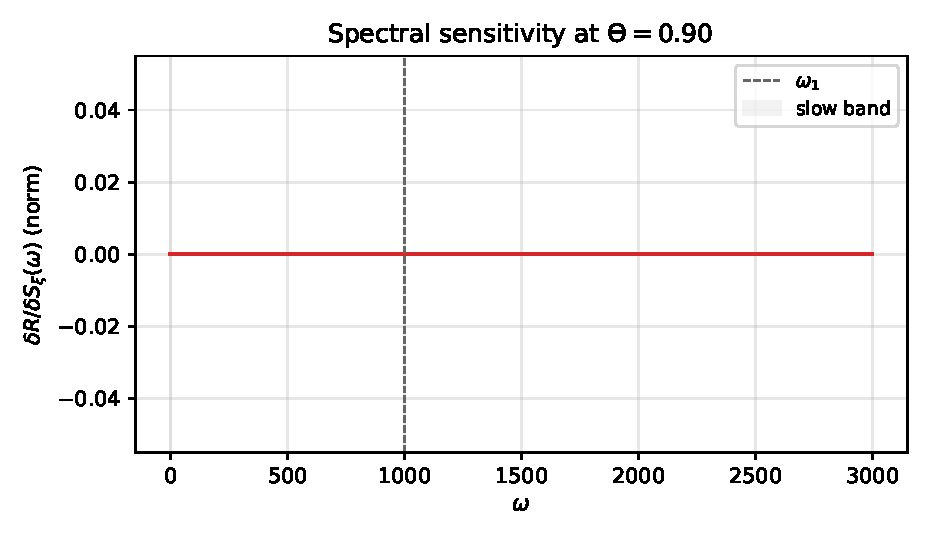
\includegraphics[width=0.72\linewidth]{figM2_true_sensitivity.pdf}
\caption{True spectral sensitivity $\delta R/\delta S_\xi(\omega)$ via a small spectral-bump experiment in a Gaussian proxy at $\Theta=0.90$ (equal-carrier enforced by re-scaling $S_\xi$ to keep $J(\omega_1)$ fixed). The slow band (shaded) marks the envelope analysis region; the carrier $\omega_1$ (dashed) is servoed.}
\end{figure}

\begin{figure}[t]
\centering
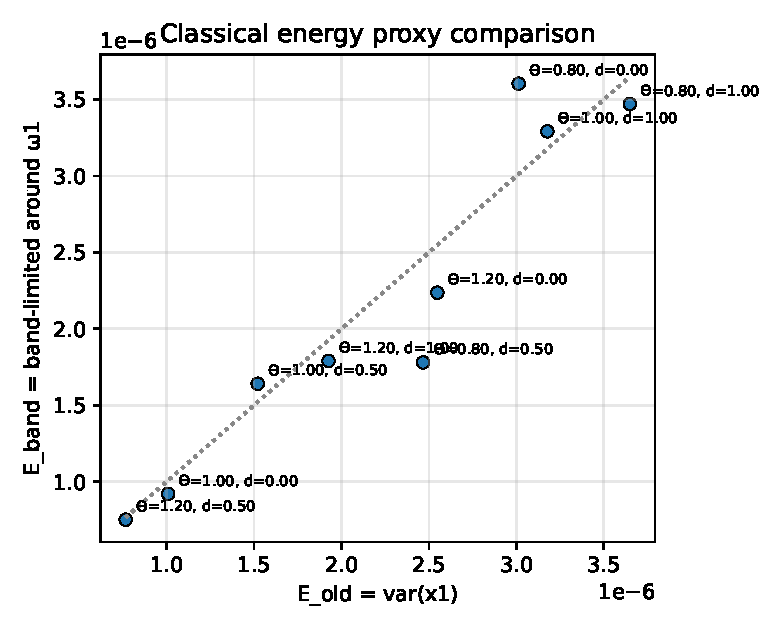
\includegraphics[width=0.72\linewidth]{figN_energy_proxy_compare.pdf}
\caption{Classical energy proxy comparison: legacy $\mathrm{var}(x_1)$ vs band-limited fast-mode energy around $\omega_1$ ($\beta=0.3$). We adopt the band-limited definition for cross-regime consistency with quantum occupancy.}
\end{figure}

\begin{figure}[t]
\centering
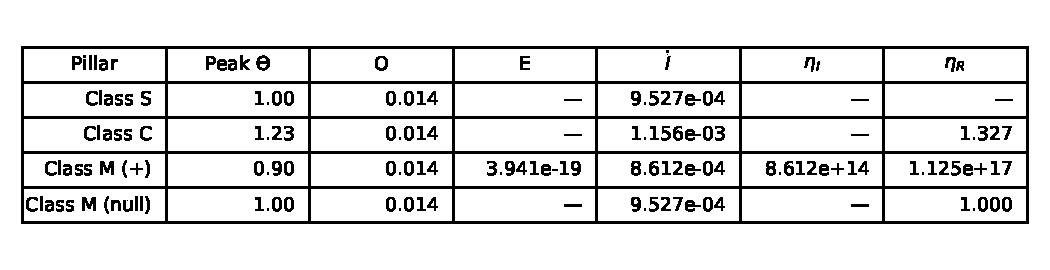
\includegraphics[width=0.7\linewidth]{figTable_frontier.pdf}
\caption{Information–Energy frontier summary. Peak $\Theta$, overlap $O$, energy $E$, information rate $\dot I$, and efficiencies $\eta_I=\dot I/E$, $\eta_R=(R_{\mathrm{env}}-1)/E$ for Classes S/C/M(±). Rows use adaptive or proxy calculations as noted in Methods.}
\end{figure}

\begin{figure}[t]
\centering
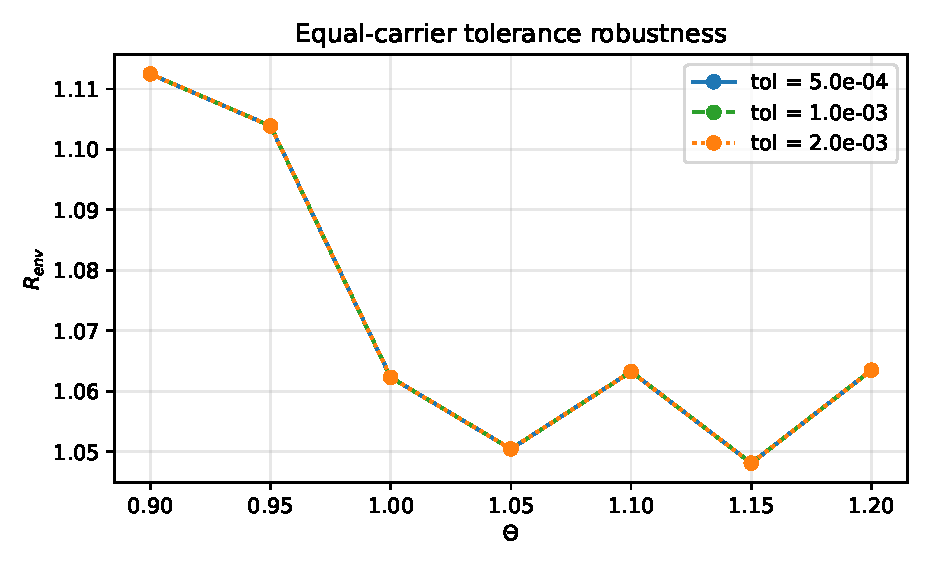
\includegraphics[width=0.7\linewidth]{figO_equal_carrier_tolerance.pdf}
\caption{Equal-carrier tolerance robustness: overlay of $R_{\mathrm{env}}(\Theta)$ for tolerances $|\Delta J|/J^\star\in\{5\times10^{-4},10^{-3},2\times10^{-3}\}$. Curves coincide within line widths, closing the \emph{more drive at $\omega_1$} loophole.}
\end{figure}

\bibliographystyle{unsrt}
\bibliography{references}
\end{document}
